\chapter{Grant Cardone: Audience, Scale, and Asset Control}

This chapter follows the School of Hard Knocks interview with Grant Cardone, curated for Video2Book by LazyingArt LLC. The mathematical content is not blackboard mathematics. It is the arithmetic of commerce: audience size, funnel conversion, lifetime drawdown, unit count, dependence, and scale. We will keep the interview's order. Cardone begins with a claim about raising capital from an audience, then moves through boredom, money reference points, people, wealth that survives, small-money management, real estate scale, sales, and finally the purpose of money after the number is reached.

\section{Audience Before Institutions}

Cardone opens before the formal interview with the claim that his group has raised \(\$1.1\) billion by crowdfunding on the internet. He immediately contrasts that with the institutional path he says he does not take: he does not begin by asking a famous investor, a billionaire, or a large equity fund to finance a project. The mechanism he wants us to see is different. First there is attention. Then there is trust. Then there is an offer. Only after that does capital move.

\[
\hbox{audience}+\hbox{trust}+\hbox{offer}
\longrightarrow
\hbox{capital}.
\]

This is not a theorem. It is the first working model of the interview. Money is not treated as a static pile. It is treated as something that can be invited through a channel that has already been built.

\begin{definition}
An \emph{audience}, in this chapter, is the accumulated group of people who know, watch, buy from, or may invest with the entrepreneur. It is not the same thing as capital, but it can become a path to capital when an offer is made.
\end{definition}

Cardone also gives the first scale reference here. He says that there are roughly \(\$80\) trillion U.S. dollars in circulation. We should treat this as his stated comparison frame, not as an independently verified monetary aggregate. Its role in the argument is to change the denominator. He does not want the listener comparing himself only with neighbors, classmates, or family stories.

\begin{equation}
M_{\mathrm{USD}} \approx \$80\text{ trillion}.
\end{equation}

The opening claim therefore has two pieces. First, capital can be raised from an audience rather than from a small committee of institutions. Second, the listener's reference point for money may be much too small.

\section{Boredom, Urgency, and the Cost of Free Time}

The first formal question is not about real estate or investing. It is about self-improvement. The interviewer asks about free time, cheap entertainment, distraction, and getting serious. Cardone answers by making boredom the enemy.

The roughness of the answer should not hide the structure. He is not offering a theory of leisure. He is describing a risk path. Free time becomes boredom. Boredom lowers standards. Lower standards change the people and places around a person. That environment produces decisions that weaken the next day.

\begin{figure}
\centering
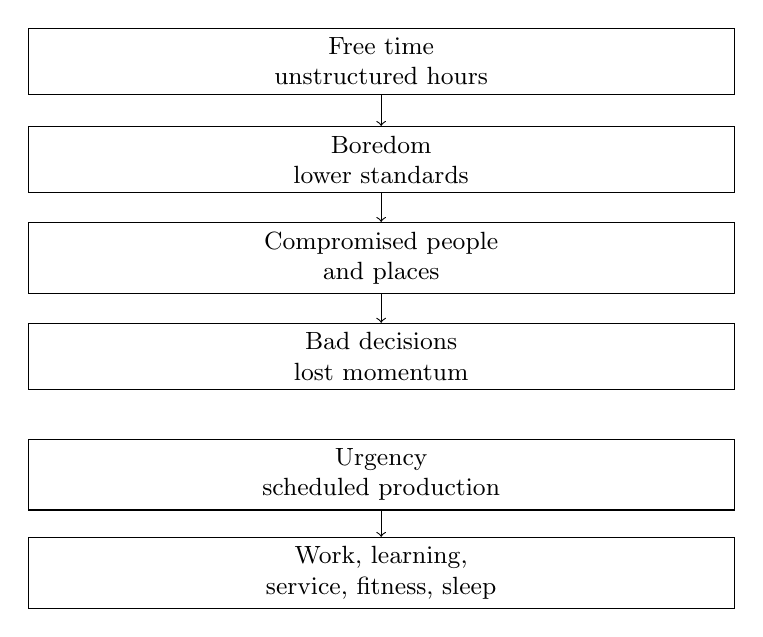
\begin{tikzpicture}[font=\small]
\node[draw, align=center, text width=.72\linewidth] (a) at (0,0) {Free time\\unstructured hours};
\node[draw, align=center, text width=.72\linewidth] (b) at (0,-1.25) {Boredom\\lower standards};
\node[draw, align=center, text width=.72\linewidth] (c) at (0,-2.5) {Compromised people\\and places};
\node[draw, align=center, text width=.72\linewidth] (d) at (0,-3.75) {Bad decisions\\lost momentum};
\node[draw, align=center, text width=.72\linewidth] (e) at (0,-5.25) {Urgency\\scheduled production};
\node[draw, align=center, text width=.72\linewidth] (f) at (0,-6.5) {Work, learning,\\service, fitness, sleep};
\draw[->] (a) -- (b);
\draw[->] (b) -- (c);
\draw[->] (c) -- (d);
\draw[->] (e) -- (f);
\end{tikzpicture}
\caption{The first operating diagram: unstructured time becomes a risk path, while urgency becomes a stabilizing path.}
\end{figure}

Cardone's answer then makes a sudden scale jump. He asks how many times a person has to make a million dollars to become a billionaire. The arithmetic identity is simple:

\begin{equation}
\$1{,}000{,}000{,}000
=
1{,}000\times \$1{,}000{,}000.
\end{equation}

But the identity is only the beginning. His spoken point is that a person does not keep every gross dollar. Payroll, taxes, retained margins, bad decisions, and losses mean that the practical number of million-dollar wins must be larger than \(1{,}000\). The arithmetic is a shock device: a billion is not one heroic million; it is repetition, retention, and survival at scale.

\subsection{Question \& Answer}

\paragraph{Question.} Why does free time become a business risk rather than simply a reward?

\paragraph{Answer.} In Cardone's account, free time is risky when it becomes unstructured drift. The danger is not idleness by itself. The danger is the sequence from idleness to boredom, from boredom to compromised surroundings, and from compromised surroundings to decisions that make tomorrow weaker. Urgency is not just emotional intensity; it is a schedule that protects the person from drift.

\section{The Million-Dollar Calculation}

The next question asks about the mindset shift around money. Cardone replies by attacking the cultural symbol of a million dollars. He asks the interviewer his age, takes \(21\) as the working number, asks how long he wants to live, takes \(80\), and divides.

Assume no further income and no inflation. Then the million dollars must be spread across \(80-21=59\) years.

\begin{align}
\hbox{remaining years} &= 80-21=59,\\
\hbox{remaining months} &= 59\times 12=708,\\
\hbox{monthly draw} &=
\frac{\$1{,}000{,}000}{708}
\approx \$1{,}412.
\end{align}

Cardone rounds the result to about \(\$1{,}400\) per month. This is the cleanest worked example in the interview. The same \(\$1{,}000{,}000\) changes meaning when it is converted from a stock into a monthly flow.

\subsection{Question \& Answer}

\paragraph{Question.} Why does \(\$1{,}000{,}000\) feel large in one frame and small in another?

\paragraph{Answer.} Because the object has changed. As a stock, \(\$1{,}000{,}000\) sounds like a large pile. As a lifetime spending stream over \(708\) months, it is roughly \(\$1{,}400\) per month before inflation, emergencies, taxes, and mistakes. The interview's point is that the word ``millionaire'' can hide the arithmetic of actual freedom.

Cardone then turns the calculation into a warning about reference points. If a person believes that a million dollars is the whole target, reaching it may produce disappointment rather than freedom. He says, in effect, that a person with no money should be cautious about having strong opinions about money. That is not a technical claim; it is an epistemic one. If the result is not working, the operating theory may be wrong.

This leads to his next mechanism: money moves through people. He demonstrates it by asking about the interviewer's cash and credit card. The point is not the card itself. The point is that another human being is the conduit.

\[
\hbox{people}
\longrightarrow
\hbox{relationship}
\longrightarrow
\hbox{trust}
\longrightarrow
\hbox{money}.
\]

Stealing is mentioned only as the rejected contrast. It can happen once and destroys the channel. Relationship is repeatable. That prepares the next distinction: being rich is not the same as being wealthy.

\section{From Poor to Rich to Wealthy}

The interviewer invokes the familiar saying that the poor get poorer and the rich get richer. Cardone interrupts the frame: rich is not wealthy. The difference is not merely more money. It is structure.

\begin{equation}
\hbox{poor}
\longrightarrow
\hbox{middle class}
\longrightarrow
\hbox{rich}
\longrightarrow
\hbox{wealthy}.
\end{equation}

The middle-class stage is described as a comfort trap: enough income and amenities to compare favorably with where the family may have started, but not necessarily enough freedom. The rich stage can still be fragile: a high salary, taxes, a larger house, a country club, retirement accounts, and visible status may all depend on the living income producer.

\begin{definition}
In this chapter, \emph{rich} means high income or visible financial comfort that can still stop when the earner stops. \emph{Wealthy} means ownership, brand, enterprise, or assets that can continue beyond the earner's immediate labor.
\end{definition}

Cardone gives two stories to make the distinction concrete. The first is Sam Walton: the founder dies, but the enterprise and family wealth continue. The second is his father, who died at \(52\). Cardone says the family's economic situation changed within about \(72\) hours because the income, the decision-maker, and the working engine stopped.

\[
\hbox{single income producer stops}
\longrightarrow
\hbox{income stops}
\longrightarrow
\hbox{household fragility appears}.
\]

\subsection{Question \& Answer}

\paragraph{Question.} What survives when the income producer disappears?

\paragraph{Answer.} In Cardone's distinction, rich income may not survive the person who earns it. Wealth survives through assets, ownership, enterprise, brand, and institutional structure. The father story is the negative proof: when the person stopped, the economic engine stopped. The Walton example is the positive contrast: when the person stopped, the enterprise did not.

\begin{remark}
Estate taxes, inheritance, and family ownership appear in the interview, but the transcript does not support a technical tax chapter. The reliable mechanism here is structural: stopped income is fragile; durable ownership is less fragile.
\end{remark}

\section{Go to Zero, Then Build Through People}

The question about the best financial advice becomes the \emph{Undercover Billionaire} story. Cardone says he was given \(\$100\) and set himself the target of building a \(\$10\) million business in \(90\) days without using his name. He presents the problem as a puzzle: how do we get from a small number to a very large number?

\begin{equation}
\$100 \longrightarrow \$10{,}000{,}000,
\qquad
\frac{10{,}000{,}000}{100}=100{,}000.
\end{equation}

The obvious move is to preserve the \(\$100\). Cardone's move is to return it. He says he wanted to go to zero as fast as possible. The phrase is intentionally provocative, but its role in the argument is precise: small money can make the person defensive. If the target is a factor of \(100{,}000\) away, guarding the original \(\$100\) cannot be the central strategy.

\subsection{Question \& Answer}

\paragraph{Question.} Why would someone return the only \(\$100\) he has?

\paragraph{Answer.} In Cardone's story, keeping the \(\$100\) keeps the problem small. It tempts him to manage scarcity rather than build reach. Returning it forces a different search: Who can I meet? What offer can I make? What can be reinvested into skill, marketing, brand, information, speed, and confidence? The claim is not that cash is useless. The claim is that the path from \(\$100\) to \(\$10\) million cannot be explained by guarding the original \(\$100\).

He then gives the reinvestment rule. Take the money earned from people and reinvest it into the business, the brand, the information base, and the operator's own capability. Later, when there is something left over, move into real assets outside the personal operating business.

That thought carries into the brand question. Cardone says that a person is building a brand anyway. His answer is not a polished branding theory. It is repeated exposure: show up, be known, tolerate being awkward, and keep returning until the world has to make room for the presence. The fight-story anecdote is rough, but the business mechanism is not violence. It is repeated appearance under resistance.

\[
\hbox{repeated appearance}
\longrightarrow
\hbox{recognition}
\longrightarrow
\hbox{trust or attention}
\longrightarrow
\hbox{opportunity}.
\]

\section{Real Estate, Scale, and Asset-Backed Lending}

The interviewer next asks about Cardone's first real estate deals and says the second deal was \(38\) units. Cardone corrects the sequence. The first deal was a single-family house. Twenty-eight days later came another single-family house. Three years later came the \(48\)-unit deal. The correction matters because the lesson was not a sudden jump. It was a three-year search after discovering a bottleneck.

The bottleneck has a name in the story: Janet. She rented the single-family house. When she moved out, there was no rent from that asset.

\begin{equation}
1\hbox{ tenant leaves }1\hbox{ unit}
\quad\Longrightarrow\quad
\$0\hbox{ rent from that asset}.
\end{equation}

This is the one-unit problem. The asset may have cash flow while occupied, but the whole stream depends on one tenant. Cardone's solution is not to make a better slogan for one-unit ownership. It is to stop buying one unit.

For the \(48\)-unit example, he gives a simple gross income calculation:

\begin{equation}
48\times \$1{,}000
=
\$48{,}000\hbox{ per month}.
\end{equation}

\begin{figure}
\centering
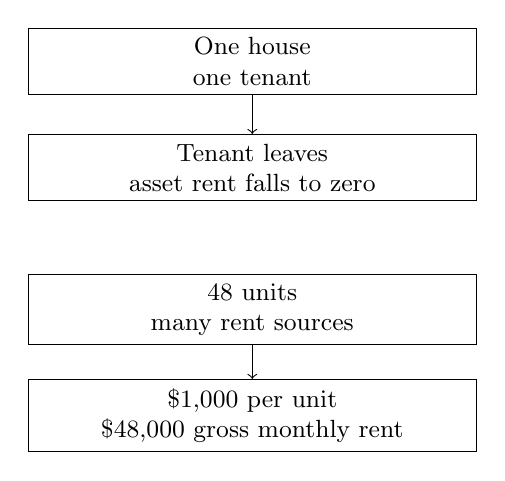
\begin{tikzpicture}[font=\small]
\node[draw, align=center, text width=.45\linewidth] (one) at (0,0) {One house\\one tenant};
\node[draw, align=center, text width=.45\linewidth] (zero) at (0,-1.35) {Tenant leaves\\asset rent falls to zero};
\node[draw, align=center, text width=.45\linewidth] (many) at (0,-3.15) {48 units\\many rent sources};
\node[draw, align=center, text width=.45\linewidth] (income) at (0,-4.5) {\(\$1{,}000\) per unit\\\(\$48{,}000\) gross monthly rent};
\draw[->] (one) -- (zero);
\draw[->] (many) -- (income);
\end{tikzpicture}
\caption{The real estate bottleneck: one tenant creates fragile income; many units create an underwritable income stream.}
\end{figure}

Cardone says the \(48\)-unit deal made him a multimillionaire. The stated numbers are:

\begin{align}
\hbox{capital raised or invested} &\approx \$350{,}000,\\
\hbox{note} &\approx \$1.9\text{ million},\\
\hbox{claimed net profit} &\approx \$3.7\text{ million}.
\end{align}

Then comes the extrapolation that changed his imagination:

\begin{equation}
10\times \$3.7\text{ million}
=
\$37\text{ million}.
\end{equation}

The point is not that ten identical deals were guaranteed. The point is that a larger unit of action changed the possible future. A \(\$200\) monthly cash-flow lesson from a single-family house taught him that income could come from assets rather than only sales. The \(48\)-unit deal taught him that the unit of scale could be large enough to change his balance sheet.

The lending lesson follows. Cardone says the bank did not lend to ``Grant'' in the ordinary personal-credit sense. It lent to the LLC or the apartment complex. We should not add loan covenants or nonrecourse terms that are not in the source. The supported claim is narrower: the income-producing entity changed the underwriting frame.

\[
\hbox{income-producing asset}
+
\hbox{entity structure}
\longrightarrow
\hbox{loan considered against the property}.
\]

\subsection{Question \& Answer}

\paragraph{Question.} Why does the \(48\)-unit property change the credit conversation?

\paragraph{Answer.} Because the object being financed is no longer just a person asking for money. In Cardone's telling, the lender can look at the apartment complex, the LLC, and the rent stream. The personal credit score is not the whole story. The asset itself becomes part of the answer.

\section{Follow the Money, Scale the Team, Close by Serving}

The real estate lesson opens into a broader scale lesson. Cardone argues that a small company can be controlled by a few employees or a few customers. With three employees, one employee can dominate the owner's attention. With thirty customers, one customer can still matter too much. With enough scale, losing one person does not break the system.

A compact way to record the mechanism is:

\[
\hbox{fragility}
\sim
\frac{1}{\hbox{number of independent customers, employees, units, or leads}}.
\]

This is not a formal law. It is the interview's repeated structure. One tenant is fragile. One income producer is fragile. A few customers are fragile. A few employees are fragile. Scale lowers dependence.

Cardone says his first business looked successful compared with his family background, but it was in a tiny vertical, could not be sold easily, could not be exited cleanly, and still depended too much on him. By contrast, he describes 10X Health as scalable to very large numbers, and his real estate business as holding about \(\$5\) billion in real estate with possible paths to \(\$10\), \(\$50\), or \(\$100\) billion if people and assets can be added.

The interview then turns into a navigation story. Cardone describes seeing very large boats clustered together and telling the captain to go back to where the money is. The story is not finally about boats. It is about using visible concentration as information. If many experienced, well-resourced actors are in one place, their location is evidence.

\[
\hbox{observed concentration of capital}
\longrightarrow
\hbox{information about opportunity or quality}.
\]

He also uses mass-demand examples. He claims the United States spends about \(\$105\) billion a year on lottery tickets, and he compares that with sports, music, concerts, and movies. He claims \(3\) million Americans have visible abs and \(22\) million are millionaires, then states the rough lesson that becoming a millionaire is more common than having visible abs.

\begin{equation}
\frac{22\text{ million}}{3\text{ million}}
\approx
7.3.
\end{equation}

The figures should be treated as Cardone's claims from the interview. Their role is to make a comparison: people badly misread probability, status, and what is actually attainable.

The sales section returns to the opening claim about audience. Cardone says \(80\%\) of what his organization does is free, and the paying portion produces very large revenue. He gives a funnel with \(16\) million online people, \(154{,}000\) product or service buyers, \(450{,}000\) interested investors, \(13{,}000\) actual investors, and \(\$1.1\) billion raised.

\begin{figure}
\centering
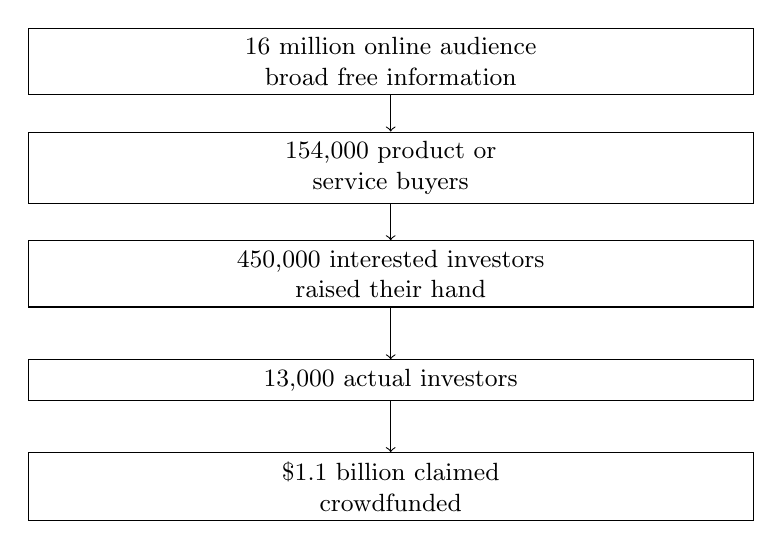
\begin{tikzpicture}[font=\small]
\node[draw, align=center, text width=.74\linewidth] (a) at (0,0) {16 million online audience\\broad free information};
\node[draw, align=center, text width=.74\linewidth] (b) at (0,-1.35) {154,000 product or\\service buyers};
\node[draw, align=center, text width=.74\linewidth] (c) at (0,-2.7) {450,000 interested investors\\raised their hand};
\node[draw, align=center, text width=.74\linewidth] (d) at (0,-4.05) {13,000 actual investors};
\node[draw, align=center, text width=.74\linewidth] (e) at (0,-5.4) {\(\$1.1\) billion claimed\\crowdfunded};
\draw[->] (a) -- (b);
\draw[->] (b) -- (c);
\draw[->] (c) -- (d);
\draw[->] (d) -- (e);
\end{tikzpicture}
\caption{A transcript-grounded funnel. The categories overlap in the telling, but the mechanism is clear: free attention narrows into buyers, investors, and capital.}
\end{figure}

The investor conversion arithmetic needs care. Cardone says the number quickly and inconsistently. The calculation is:

\begin{equation}
\frac{13{,}000}{450{,}000}
\approx
0.0289
=
2.89\%.
\end{equation}

So the arithmetic supports about \(2.9\%\). The spoken ``2.8\%'' is close; the spoken ``0.28\%'' is not.

For product buyers out of the online audience:

\begin{equation}
\frac{154{,}000}{16{,}000{,}000}
\approx
0.0096
=
0.96\%.
\end{equation}

That is approximately \(1\%\), even though the transcript describes the figure as less than one tenth of one percent. The useful point remains: a very small buying fraction can still produce a large business if the audience is large enough.

Repeat purchase is the closing mechanism. Cardone says that \(45{,}000\) of \(154{,}000\) buyers bought three, four, five, six, seven, or eight things.

\begin{equation}
\frac{45{,}000}{154{,}000}
\approx
0.292
=
29.2\%.
\end{equation}

That supports his spoken ``like \(30\%\)'' claim. It also clarifies his definition of closing. Closing is not framed as trapping the buyer. Closing is when the buyer can finally be served, and the real test is whether the relationship continues.

\begin{table}
\centering
\begin{tabular}{p{.22\linewidth}p{.32\linewidth}p{.34\linewidth}}
\hline
Anecdote & Claim & Mechanism\\
\hline
Father's death & Income-rich can stop suddenly & Wealth must survive the worker\\
\hline
Undercover Billionaire & \(\$100\) is too small a frame & People and reinvestment replace defensive management\\
\hline
Janet moves out & One unit can go to zero rent & Unit count reduces tenant dependence\\
\hline
Yacht cluster & Go where money already is & Capital concentration carries information\\
\hline
Sales funnel & Small conversion can still scale & Large audience times small percentage can be large\\
\hline
\end{tabular}
\caption{The main stories separated into anecdote, claim, and mechanism.}
\end{table}

\section{Summary: Production, Discipline, and What Money Is For}

The final turn is personal again. The interviewer asks about Cardone's lowest period: baseball not working out, drugs, the wrong crowd, and the long process of getting his life back on track. Cardone says it took ten years to lose and about three years to clean up the damage. He changed friends, changed places, made amends, showed up early, stayed late, and spent his time working, learning, helping, or sleeping.

This returns us to the beginning. Boredom was the first enemy, and it remains the enemy. Cardone says he still avoids late-night situations that are bad for him. He tells the Jamie Foxx birthday-party story to make the point: for him, a \(2{:}30\) a.m. club invitation is not neutral. It belongs to the wrong operating environment.

He then says that a person does not need to hit bottom; the person can manufacture the dissatisfaction needed to move. Even here, the mathematics is implicit. He keeps looking at larger objects, larger boats, larger costs, larger staffing requirements, and asks what would have to be produced to reach them. The calculation keeps him in a game of production rather than a game of destruction.

The last claim is about what money is for. Cardone argues that real obligations require money: family, schools, hospitals, churches, employees, businesses, and assets. Good feelings do not buy groceries. In the interview's own rough style, nobody takes happy moments at the register.

\[
\hbox{production}
\longrightarrow
\hbox{income}
\longrightarrow
\hbox{reinvestment}
\longrightarrow
\hbox{real assets}
\longrightarrow
\hbox{durable capacity to choose and help}.
\]

At the end, his advice to the younger interviewers is not to stack cash forever. First invest in yourself and the business; then, once the operating engine exists, put money into a third thing, a real asset outside the self and the business. In the interview's time frame he names Austin real estate and predicts an unusually strong buying opportunity, even saying some assets may trade around \(40\%\) below the last buyer's price. That should be read as Cardone's forecast in the interview, not as a general timeless guarantee.

The chapter's mathematical spine is compact but serious. A million dollars becomes roughly \(\$1{,}400\) a month when divided over a young lifetime. A billion is at least \(1{,}000\) million-dollar units before taxes and losses. One tenant leaving one house can make rent zero. Forty-eight units at \(\$1{,}000\) per month produce \(\$48{,}000\) in gross monthly rent. \(\$3.7\) million repeated ten times becomes \(\$37\) million. \(13{,}000\) investors out of \(450{,}000\) interested people is about \(2.9\%\). \(45{,}000\) repeat buyers out of \(154{,}000\) buyers is about \(29.2\%\).

The doctrine that emerges is not a textbook finance theory. It is a source-grounded operating rule: stop treating money as a symbol, and study the channels by which it moves through people, offers, trust, scale, entities, and assets.